% [3~v\textsuperscript{o}]
\count\Bfootins=1200
\count\Cfootins=1200
\count\Afootins=1200
\pstart
\begin{wrapfigure}[10]{l}{0.4\textwidth}                    
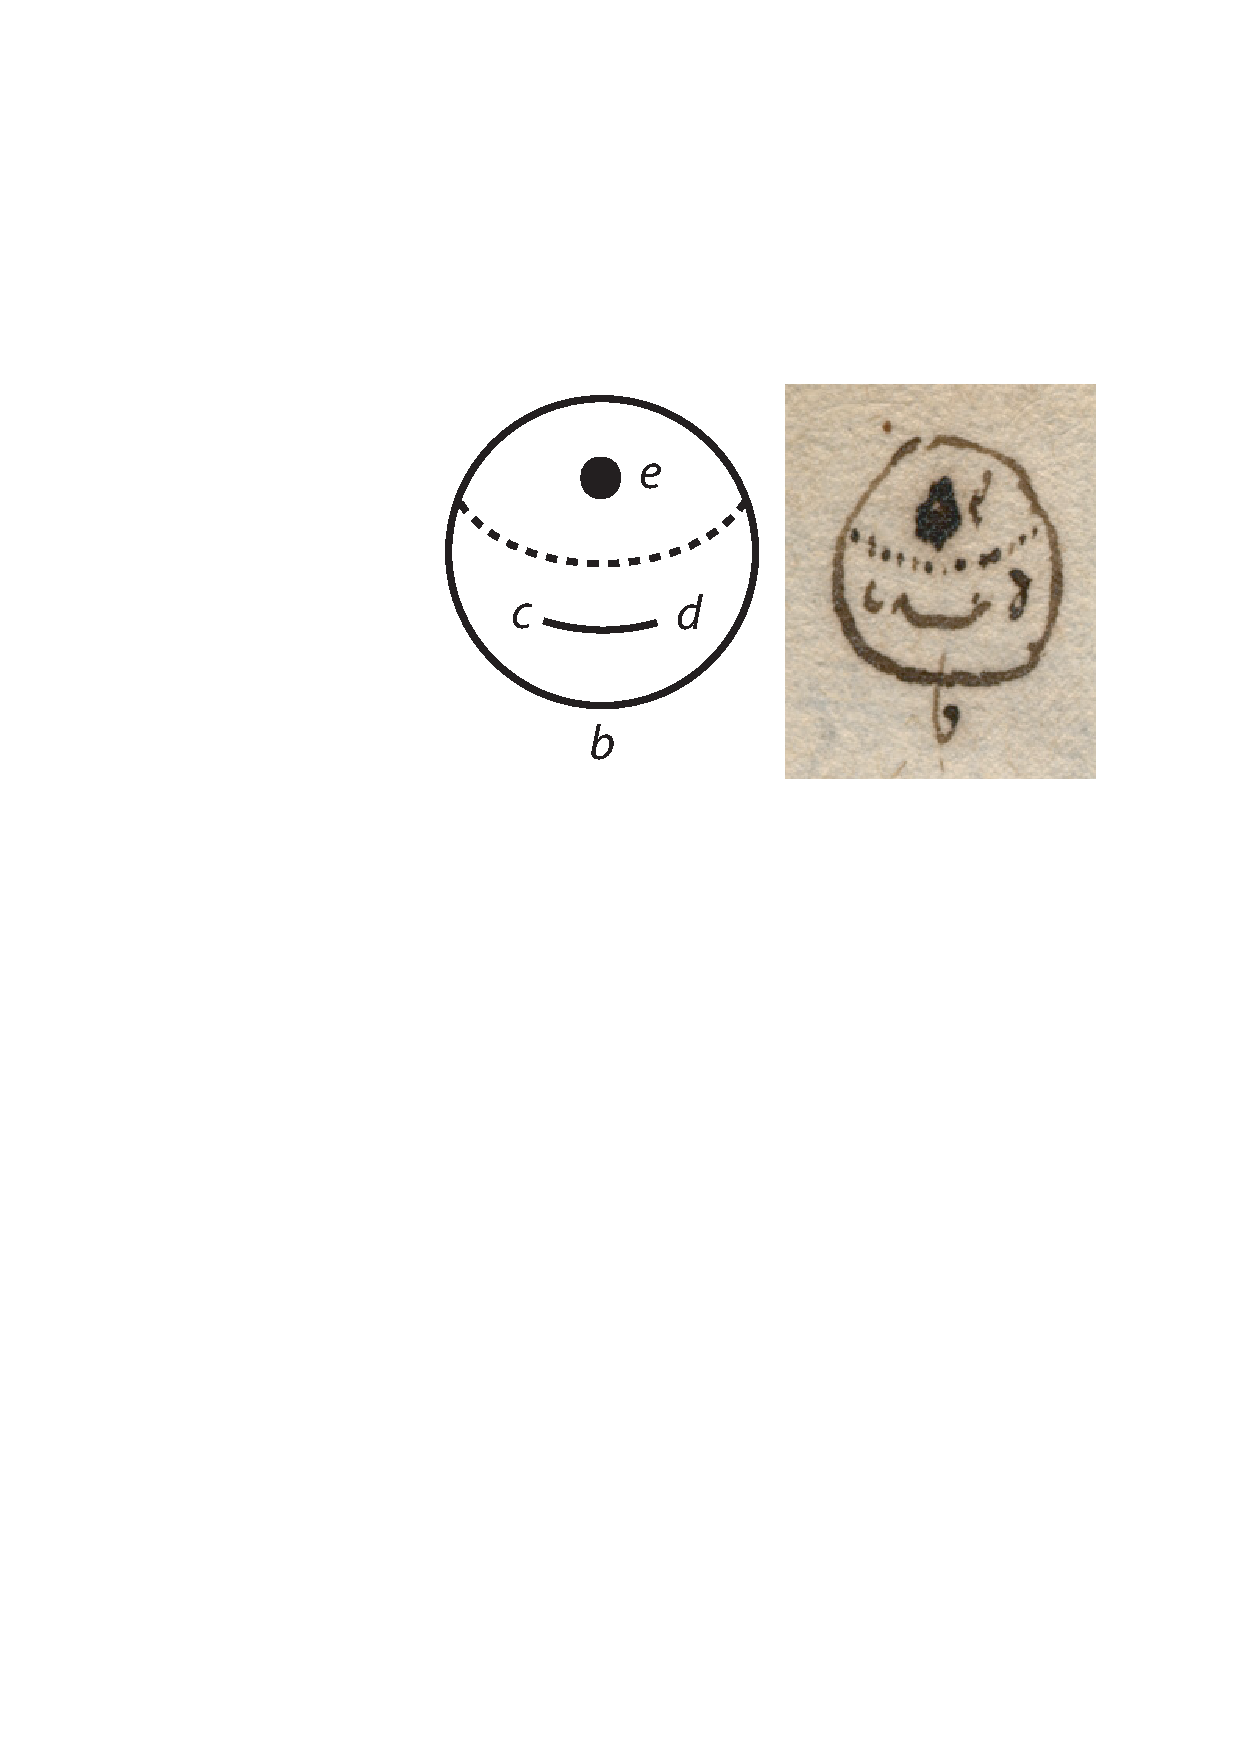
\includegraphics[trim = 0mm -3mm -5mm 0mm, clip,width=0.4\textwidth]{images/lh0040104b_003v1.pdf}\\
\rule[0mm]{19mm}{0mm}[\textit{Fig. 2}]
%\caption{Bildbeschreibung}
\end{wrapfigure}
In vituli junioris corde notavi manifeste parietem medium com\-poni ex duobus ventriculorum parietibus, item dextri $b$ ventriculi cavitas erat inflexa, ut $cd,$ et sinistri $a$ erat triangularis $e.$ Item nullae adhuc erant valvulae arteriae venosae nec venae cavae \edtext{imo erant earum rudimenta,}{\lemma{imo [...] rudimenta}\Bfootnote{\textit{erg. L}}}
sed in dextro sinu illud tuberculum rotundum, quod duas valvulas conjungebat in priori corde, in hoc erat instar columnae conjungens medium parietem cum pariete externo dextri lateris, ita tamen ut adhaereret medio parieti versus basin, et externo versus mucronem. Item valvulae aortae et venae arteriosae erant perfecte factae, ut in priori mucro sinistri lateris multo longius producebatur quam dextri, et erat longe magis cavum in fine, apertum erat illud sinistrum latus a dextro amplexum fuisse sic complicatum, et poterat adhuc explicari. Caro erat mollior, multo quam praecedentis. Latus dextrum erat superior et omnino versus sternum
\edtext{positum, atque}{\lemma{positum,}\Bfootnote{\textit{(1)}\ latus \textit{(2)} atque \textit{L}}}
auricula dextra etiam superior. 
\pend 
\pstart  Gula magis versus sinistrum latus asperae arteriae\label{aspera} descendebat quam versus dextrum ab origine et aspera arteria habebat in posteriori parte quasi cristam quandam cui gula incumbebat\setline{21} a sinistris.
\pend%
\vspace{1.5em}
\pstart% 
\centering 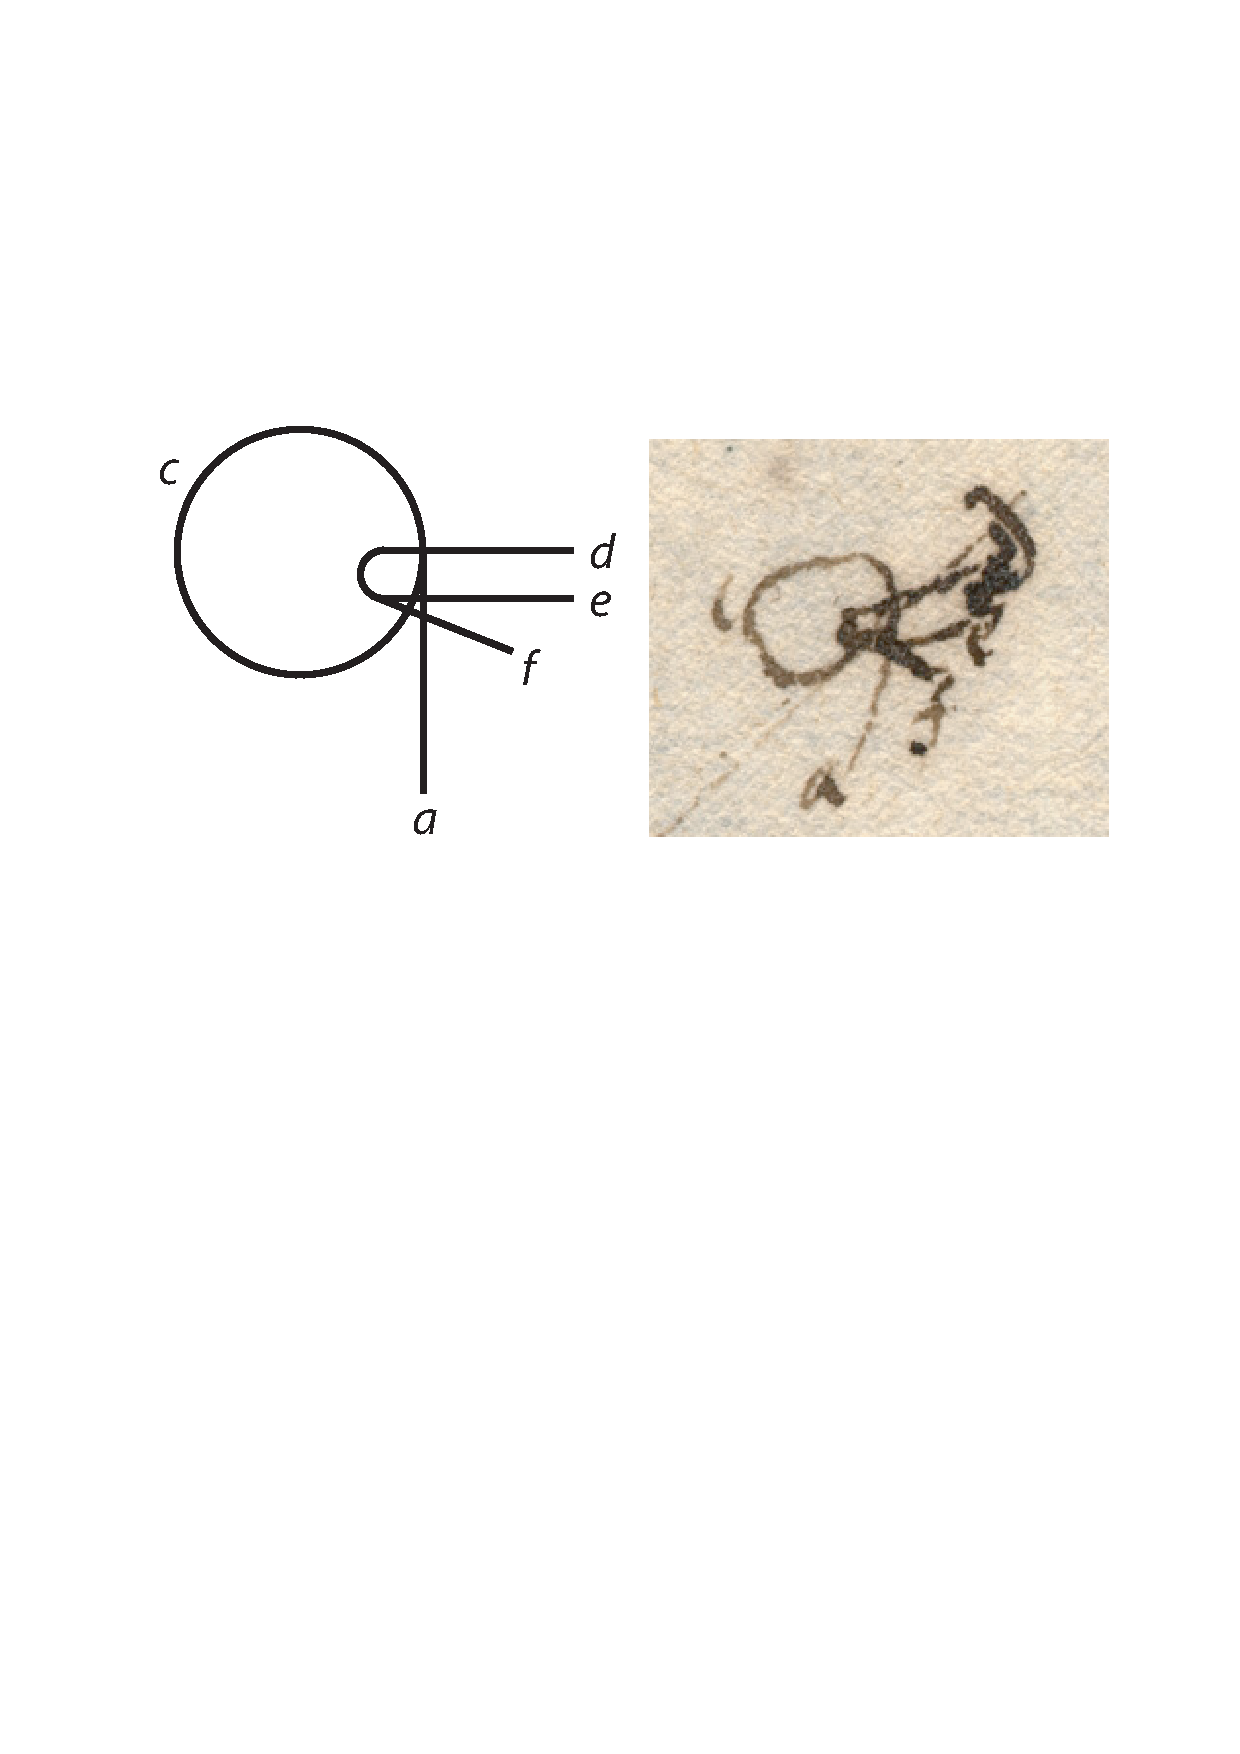
\includegraphics[trim = 0mm -3mm 0mm 0mm, clip,width=0.59\textwidth]{images/lh004014b_003v2.pdf}\\
\centering[\textit{Fig. 3, gestr.}]
%\caption{Bildbeschreibung}
\pend
\pstart
[\textit{Folgender kleingedruckter Text im Ms. gestrichen:}]
\edtext{}{\lemma{}\Afootnote{\textit{Am Rand:} (+ haec deleta erant +)\vspace{-4mm}}}%
\footnotesize%
Vena arteriosa sic initio a cava procedit per spiram $abc$ et dividitur in tres ramos, quorum 2 $d$ et $e$ ad utrumque pulmonem tertius $f$ cum aorta confunditur, estque canalis ille medius, de quo libri, qui paulum in adultis obliteratur.
\pend
\vspace{0.5em}
\pstart
Notavi hic venam umbilici esse ejusdem fere compositionis atque tunicae arteriae. Hic videtur initio cava fuisse in anteriore parte atque inde ascendendo per sinistram partem supra cor transiisse versus spinam, atque ibi in arteriam magnam descendisse (simulque in pulmones, ut vena arteriosa existens) ramos emisisse. Tuncque arteria venosa etiam \edtext{in anteriore}{\lemma{in}\Bfootnote{\textit{(1)}\ ex \textit{(2)}\ anteriore \textit{L}}} parte, sed magis versus latus \edtext{dextrum descendendo}{\lemma{dextrum}\Bfootnote{\textit{(1)}\ descendere \textit{(2)}\ descendendo \textit{L}}} cor fuisse ingressam, atque inde versus sinistram ascendisse rursum in aortae partem ascendentem simulque ramum\label{ramus} in venam arteriosam demisisse, qui sensim factus est ramus aortae descendentis venae cavae truncus ascendens dirigebatur in sinum inferiorem auriculae sinistrae per laxam valvulam ibi positam, atque inde in sinistrum ventriculum cum arteria venosa quae multis ramis in sinum sinistrum ex pulmone descendebat, qui rami faciebant superiores anfractus auriculae sinistrae. Solus igitur ramus cavae descendens a capite in dextrum sinum ingrediebatur imo etiam ascendens prius eo ibat quam ad sinistrum, sed erat vas insigne (simplici tunica praeditum) in summo medii parietis inter ingressum cavae et arteriam venosam a dextro ventriculo supra sinistram auriculam ad truncum aortae descendentis se applicans, nempe erat alius ramus cavae ascendentis. 
\pend 
\pstart Circa 1\textsuperscript{mum} hepar juvenis vituli haec notavi, 1\textsuperscript{o} vena umbilicalis ita in hepar immergebatur, ut hepar supra revolveretur, et quasi fossam faceret duorum digitorum quasi profunditate, in quam venam umbilicalem admittebat, ligamentum e peritoneo suspensorium dictum, venae quoque umbilicali adhaerebat, videbaturque distinguere mediam partem ejus hepatis qui fuerat antequam traxisset umbilicum, nempe forma hepatis erat maxime irregularis, in dextro enim latere quadruplo vel quintuplo major erat quam in sinistro, nempe quod ventriculus ex sinistra parte illum repulerat, eratque ejus quidam lobus $d$ in dextro latere, cui apparebant etiam ligamenti suspensorii vestigia quae recta per $a$ $c$ super hepar transibant, infra vero suspicor ea ab accedente ventriculo rupta fuisse, et videbantur ita deflexisse, ut ex $c$ ad $i$ vasa fellis, et ab $i$ ad $d$ lobum dextro ascititium procederent, unde patet fellis vesicam $e$ genitam fuisse, cum hepar magna vi cresceret, tumque illam non tam in dextro latere, ut est in adultis, sed in ea parte, quae tum erat hepatis\hfill media\hfill genitam\hfill fuisse,\hfill et\hfill in\hfill loco\hfill a\hfill cava\hfill maxime\hfill remoto.\hfill Manifestum\hfill erat\hfill etiam
\pend
\newpage
\pstart\noindent venam portam totam a vena umbilicali procedere, ductus enim ab umbilico ad portas hepatis erat praecipuus aliusque erat inde ad lobum dextro ascititium, etiam insignis, ex quo confirmatur mea conjectura, nempe istum lobum quasi fractum et disjunctum fuisse ab ea parte hepatis in qua erat umbilicus superveniente ventriculo. Venae autem portae exitus ad mesenterium erat praecise inter istum lobum et umbilicum, ut fel, sed supra inter fel et truncum cavae, adeo ut praecise ex loco medio partis inferioris hepatis emergeret.
\pend
\pstart
Nihil circa fel notare potui, nisi quod videretur ex humore in cavae ramis concocto conflari, quoniam ramus insignis e cava supra illum absorbebatur; \edtext{praeterea}{\lemma{}\Afootnote{\textit{Am Rand:} (+ NB +)\vspace{-4mm}}} exonerabatur in magnum quoddam vas, quod puto fuisse duodeni intestini partem juxta portas hepatis positam, quanquam ejus ductus in substantiam hepatis magis pateret. Pulmones erant in duas partes ita divisi, ut sinistra paulo minor quam dextra videretur vasa omnia sinistrae partis egrediebantur ex eodem loco fere in anteriore parte vasa autem dextrae \edtext{[partis]}{\lemma{partes}\Bfootnote{\textit{L \"{a}ndert Hrsg.}}} egrediebantur quidem simul etiam ex eodem loco, sed non tam ex anteriore parte, imo potius ex medio, nisi forte unus aut alter ramus qui jam excisi erant, magis ex anteriore parte procederent. Videbatur ergo dexter lobus in duos rursus divisus, sed et hi in plures, ut etiam sinister erat in plures dissectus, ita tamen ut cum in dextro tum in sinistro, esset una pars praecipua et magis continua quae deorsum tenderet, reliqua tantum modo ex sequaci carne conflata videbantur excrevisse ad thoracis cavitatem replendam.
[4~r\textsuperscript{o}]
\pend
%\count\Bfootins=1500
%\count\Cfootins=1500
%\count\Afootins=1500